\documentclass[11pt]{amsart}
\usepackage{geometry}                % See geometry.pdf to learn the layout options. There are lots.
\geometry{letterpaper}                   % ... or a4paper or a5paper or ...
%\geometry{landscape}                % Activate for for rotated page geometry
%\usepackage[parfill]{parskip}    % Activate to begin paragraphs with an empty line rather than an indent
\usepackage{graphicx}
\usepackage{amssymb}
\usepackage{amsthm}
\usepackage{amsmath}
\usepackage{mathtools}
\usepackage{rotating}
\usepackage{epstopdf}
% \usepackage{multirow}
\usepackage{xcolor}
\usepackage{array}
\DeclareGraphicsRule{.tif}{png}{.png}{`convert #1 `dirname #1`/`basename #1 .tif`.png}

% %%%%%%%%%%%%%%%%%%%%%%%%%%%%%%%%%%%%%%%%%%%%%%%%%%%%%%%%%%%%%%%%%%%%%%%%%%%%%
% user-defined environment, operators, commands, etc.
\newenvironment{conditions}
  {\par\vspace{\abovedisplayskip}\renewcommand{\arraystretch}{1.5} \renewcommand{\tabcolsep}{0.2cm}\begin{tabular}{>{$}l<{$} @{${}={}$} l}}
  {\end{tabular}\par\vspace{\belowdisplayskip}}

\DeclareMathOperator*{\argmin}{argmin}
\DeclareMathOperator*{\argmax}{argmax}

\newtheorem{condition}{Condition}
\newtheorem{hypothesis}{Hypothesis}

\newcommand{\he}[2][{}]{\ensuremath{{#1}^{\circ #2}}}
\newcommand{\densematrix}[3]{%
    \ensuremath{\begin{pmatrix}
        #1_{11}  & #1_{12}    & \cdots    & #1_{1#3}    \\
        #1_{21}  & #1_{22}    &           & \vdots      \\
        \vdots   &            & \ddots    &             \\
        #1_{#21} & \cdots     &           & #1_{#2#3}
    \end{pmatrix}}}
% %%%%%%%%%%%%%%%%%%%%%%%%%%%%%%%%%%%%%%%%%%%%%%%%%%%%%%%%%%%%%%%%%%%%%%%%%%%%%

\title{A General Approach for Learning Constitutive Relationships (Physical Laws) from Neural Networks}
\author{Andrew Temple}
\author{Matthew Miller}
\author{Maria Quintana-Hernandez}
\author{Aaron Stebner}
\author{Peter Collins}
\author{Branden Kappes}
%\date{}                                           % Activate to display a given date or no date

\begin{document}
\maketitle
%\section{}
%\subsection{}

\section{Abstract}\label{Abstract}

While it is possible to extract equations from various machine learning strategies such as artificial neural networks that relate the independent variables (inputs) to a dependent variable (output), these equations do not naturally reflect known physical phenomena. Here, we present a general approach to learn and produce natural (and perhaps well-known) constitutive relationships (physical laws) from neural networks. The approach is presented in this paper as a comparison of mathematical series expansions of the optimized formula from neural networks and a learned/optimized physical relationship, whether or not known a priori.
% Only certain types of expansions permit convergence to solutions; a gap that must be addressed.
This linkage between the powerful infrastructure of neural networks and the fundamental physical phenomena and laws has many implications that will be introduced. General expansions for many physical phenomena are presented.


\section{Introduction}\label{introduction}

With apologies to the Bard of Avon, \\

\vspace{2mm}
\noindent
\textit{Two methods, both alike in dignity, \\
In fair sciences, where we lay our scene. \\
From ancient elegance break to methods mutinous, \\
Where machine learning makes physical laws unclean, \\
From forth the noble loins of these two foes\\
A pair of cross-term'd numbers seek their place;\\
Whose serial expansions, equally covariant\\
Do with their projections, bury their parents strife.\\
Our fearful assessment of their dual-space truth,\\
And the continuance of their parents, sage,\\
Which, for their children's union, sought to achieve,\\
Is now the two hours' traffic of our stage;\\
The which, if you with patent eyes attend,\\
What here shall miss, our toil shall strive to mend.\\}

\vspace{2mm}

With the proliferation of increasingly powerful machine learning strategies, and their promise of the automatic discovery of new physics, phenomena, properties, and correlations, it is seductive to trust machine learning to solve our most complex problems. The unintended consequence of relinquishing one's data to machine learning is that our native physical understanding of currently-understood phenomenon may atrophy, and our development of descriptions of new physics may stagnate.  These risks could have profound impacts on numerous scientific fields. Consider the instruction of machine learning, where students, and hence future scientists, engineers and educators, may, unintentionally, understand machine learning to be a cudgel against which every problem which has a solution falls. When one tool is so powerful as to render other methods seemingly obsolete, it is natural to "disarm" oneself of the tools that seem obsolete.  Yet, such tools are not obsolete.  Various physical phenomenon are exceptionally well described by laws (the laws of Thermodynamics, kinetics, motion, ...) or theories (e.g., dislocations which underpin our understanding of strength in metals and alloys).  Those laws and theories permit us to creatively explore spaces where data does not exist, hypothesize, theorize, and test our hypotheses.  In the absence a mastery of our understanding of physical processes, the scientific method in its currently and widely accepted form, becomes harder to apply.  Thus, we must: retain mastery of current theory; postulate logically new theories; and leverage mathematical powers to understand complex hyperspaces describing n-variables. \\

The problem of whether to apply our most powerful tools in our analytical arsenal to a problem, or rigorously develop theories or calculate previously unknown physical constants seems to become an either-or problem.  Much like the houses of the Montagues and Capulets in Shakespeare, the tools of Machine Learning and Phenomenological Relationships seem irrenconcilable. Yet, the problem lies with neither approach (both alike in dignity), rather it stems from two very human limitations. Firstly, we have great difficulty interpreting problems in higher-order space.  It is easy to understand problems which have a single independent variable against which a phenomena depends, resulting in y-x plots of data.  It is not much harder to understand problems which have two independent variables against which a phenomena depends, as these can be represented in Euclidean space, and with imagination we can understand problems with three independent variables (say x,y and time) against which a phenomena (say, z=f(xy,t)) depends.  Beyond this, we lack tools to understand or visualize an n-variable hyperspace.  Secondly, we can develop an implicit bias when wrestling with mathematical expressions, and may begin to believe that one (and hence, only one) functional expression can be used to fit a relationship.  We develop mathematical "favorites", tools that, quite rationally, we turn to when solving certain problems.  We turn to these expressions for two reasons: they work, and they are reduced to the simplest form possible.  In materials science, against which the framework presented in this paper has been conceived and for which a simple discipline-specific problem will be tackled, it is common to turn to the Arrhenius relationship for phenomena which have temperature dependencies.  This simple form, $A=A_O\exp{-\frac{Q}{kT}}$, is taught in extensively in a wide variety of classes, and yet, there is nothing in nature that dictates the exponential form be used.  It is used because it is the simplest mathematical expression to fit the observed data.  And yet, it could be expanded, in, e.g., polynomial form... \\

If this recognition that our most trusted expressions can be re-written in polynomial form, then so too must the reduced functions describing the most flexible and powerful neural networks out there.  The next logical step is to postulate that these expanded forms of different representations of the same physical phenomena can be compared, and assessed for their self-similarity, providing a \textit{translation} between one form and another.  A Rosetta Stone, if you will, where the mathematical functions (i.e., the language) in one reference frame can be translated and assessed for equivalency to the mathematical functions of the second reference frame\footnote{It is critically important to recognize that while we are describing the translation between two reference frames, that of Machine Learning and that of Constitutive Laws of certain physical phenomena, there is no limitation to the number of reference frames (languages) among and between which the relationships can be established...which provides a way for different disciplines, describing the same phenonmena using different expressions, a way to translate their work - EXPAND THIS IN CONCLUSIONS, ... different data, equipment, labs, ...}.\\

The precursors to this thought process began when H.L. Fraser et al. began conducting so-called virtual experiments, which permitted a well-trained neural network to be probed to determine the influence of one variable on a physical property while all of the other potential independent variables were artificially held at their average values [refs]. These virtual experiments were slices through an n-dimensional hyperspace, and it became obvious that the lower dimension slices could be described using simpler functions than the full neural network.  This early work was built upon the initial efforts by H.K.D.H. Bhadeshia to solve complex materials science problems using artificial neural networks [refs] and the work of D.J.C. MacKay [refs] to incorporate Bayesian statistics and feedback loops.  Following this prior work, with the assumption that a mapping was possible between the basis vectors of the n-variable hyperspace equally represented by the expansion of terms of an artificial neural network and the basis vectors representing the physical processes, Ghamarian and Collins, seeking to establish a constitutive equation for the room temperature yield strength of a titanium alloy given variations in its compositional and microstructural states, applied a hybrid artificial neural network-genetic algorithm method that optimized the unknowns in a postulated physically-based equation, testing the optimized physically-based model against slices through hyperspace function representing the neural network model and the data [refs]. This latter effort was quite inefficient, but resulted in a solution that proved, in subsequent work, to be generalized for multiple different variations of processing and with compositional variations [refs].   \\

This previous work strongly suggests that the hypothesis we propose below is valid, and that a more fulsome mathematical treatment is merited and which is the subject of this paper.  We recognize that this approach lies neither fully in a mathematics space nor in an engineering/science space. Consequently, we aim to provide both sufficiency of the derivations and sufficiency of motivation and impact, so that the paper is accessible to readers of various communities.  While we demonstrate the approach on a materials science problem, we hope that the general applicability will be apparent, as it is easy to imagine this approach impacting a diverse range of disciplines, including: genetics, public health, biological sciences, earth sciences, information sciences (including signals analysis), physical sciences, applied variants thereof (medicine, environmental activities, engineering), space sciences, and economics.  We finally include an appendix that includes the expansions of the activation functions and the generating functions of common functions that form the basis of some relevant physics.  We recognize that this appendix is far from complete, but hope that the logic presented will permit those interested in identifying and developing additional functions as the specific applications demand.\\

\textbf{\textit{The hypothesis}}: We hypothesize that the physics of an arbitrary and complex process can be extracted by fitting the polynomial expansions of known/postulated/potential physical relationships to the polynomial coefficients of a polynomial series expansion of an arbitrary and complex neural network.\\

\textcolor{red}{NOTE:  DISCUSS IN TEXT - if any physical constants are known, they can be directly entered into the expansions...}





\section{Methods}\label{methods}

Fully dense neural network (NN) architectures, such as the one shown in Figure~\ref{fig:nn-1}, perform a sequence of affine transformations, ${\bold z}_i \leftarrow \boldsymbol\theta_i {\bold x}^{(i)}$, followed by element-wise functional operations, $\sigma({\bold z}_i)$ to introduce non-linearity at each layer; that is, each layer stretches and distorts the underlying space.
\begin{figure}[htbp]
\begin{center}
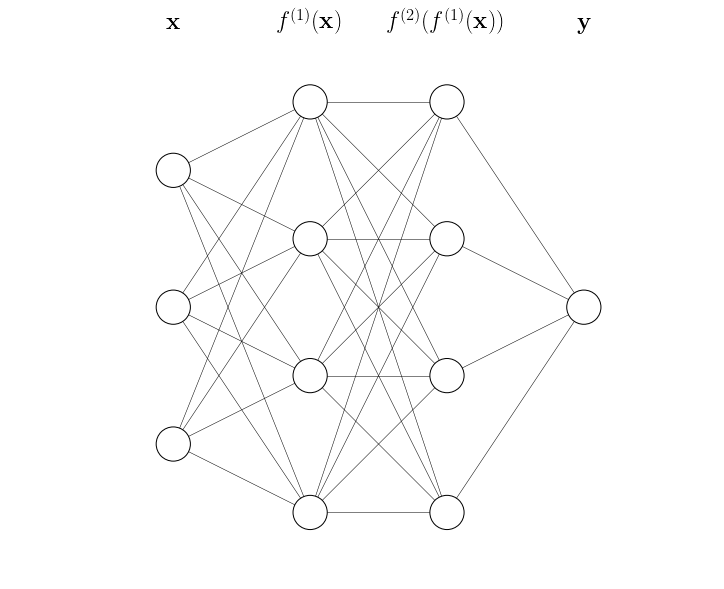
\includegraphics[width=0.4\textwidth]{fig/neural-network-01}
\caption{Schematic view of a fully dense neural network. Each sequence of affine and non-linear transformations are captured in the function, $f_i({\bold x}): {\bold x}^{(i+1)} \leftarrow \sigma(\boldsymbol\theta_i {\bold x}^{(i)})$}
\label{fig:nn-1}
\end{center}
\end{figure}

The resulting network,
\begin{equation}
	f(x) = \sigma(\boldsymbol\theta_n \sigma(\boldsymbol\theta_{n-1} \sigma(\ldots \boldsymbol\theta_2 \sigma(\boldsymbol\theta_1{\bold x}))))
	\label{eqn:nn analytical form}
\end{equation}
is an arbitrary function generator, but at present, the network weights $\boldsymbol\theta_i$ can not map back to analytic forms that capture and describe the underlying physics. There are, however, many such mappings through polynomial series expansions,
\begin{equation}
	f(x) = \sum_{n=0}^\infty a_n x^n
\end{equation}

We hypothesize that the physics of a process can be extracted by fitting the polynomial expansions of known physical relationships to the polynomial coefficients of a polynomial series expansion of Equation~(\ref{eqn:nn analytical form}). \\
\\*



%Beginning of softmax derivation 1/7
The Softmax activation function is given in Equation (\ldots)

\begin{equation}
	\sigma(\bold z)_i =
	\frac{e^{z_i}}{\sum\limits_{j=1}^k e^{z_j}}
\end{equation}

The partion function, $\bold Z$, is defined below as
\begin{equation}
	\bold Z = \sum\limits_{j=1}^k e^{z_j}
\end{equation}
The series expansion for the exponential is given by the following
\begin{equation}
	e^{z_{i}} = \sum_{k=0}^{\infty}\frac{1}{k!} z_{i}^{k}
\end{equation}
Therefore
\begin{equation}
	\sigma(\bold z)_i = 
	\sum\limits_{k=0}^{\infty} \alpha_{k}z_{i}^{k}
\end{equation}
Where $\alpha_k = \frac{1}{{\bold Z}k!}$ is the generating function for the Softmax
%End of softmax derivation 1/7


The ReLU (rectified linear units) function is another commonly used activation function and is given below in Equation~(\ref{eqn:ReLU}):
\begin{equation}
	f(x) =
	\begin{cases}
		x, & \text{if}\ x > 0 \\
		0, & \text{otherwise}
	\end{cases}
	\label{eqn:ReLU}
\end{equation}

The variable $\bold x$ in Equation~(\ref{eqn:nn analytical form}) represents a column vector containing $\boldsymbol n$ input elements, and thus, the output from each node will be multplied by the respective weight before the application of the subsequent activation function.

e.g.,
\begin{equation}
	\bold z =
	\theta^{(1)} \begin{bmatrix}
				x_{1} \\
				x_{2} \\
				\vdots \\
				x_{n}
			\end{bmatrix}
	\Rightarrow \begin{bmatrix}
					\theta_{11} x_{1} + \theta_{12} x_{2} + \ldots \theta_{1n} x_{n} \\
					\theta_{21} x_{1} + \theta_{22} x_{2} + \ldots \theta_{2n} x_{n} \\
					\vdots \\
					\theta_{m1} x_{1} + \theta_{m2} x_{2} + \ldots \theta_{mn} x_{n} \\
				\end{bmatrix}
\end{equation}

and $\boldsymbol\sigma (\bold z)$ serves as the input of the next layer in the network, where $\bold z = (\boldsymbol\theta^{(1)} \bold x)$.

The generating function for the ReLU is given in Equation~(\ref{eqn: ReLU generating function}) and it is dependent on both the input variables and the network weights.
\begin{equation}
	\ a_n =
		\begin{cases}
			1 & \bold z > 0 \\
			0 & \text{otherwise}
		\end{cases}
	\label{eqn: ReLU generating function}
\end{equation}

The linear generating function is given in Equation~(\ref{eqn: linear generating function}) and it is only dependent upon $\bold n$.
\begin{equation}
	\ a_n =
		\begin{cases}
			1 & \bold n = 1 \\
			0 & \text{otherwise}
		\end{cases}
	\label{eqn: linear generating function}
\end{equation}

Although ReLU (rectified linear units) have become a more common activation function, its discontinuity at $x = 0$ requires an infinite series to fully capture the behavior at this transition. However, the softplus function,

\begin{equation}
	f(x) = log(1+e^x)
\end{equation}

The series expansion for the exponential
\begin{equation}
	e^x = \sum_{k=0}^\infty \frac{x^k}{k!}
\end{equation}
where, $a_k = \frac{1}{k!}$, can be expressed as
\begin{equation}
	e^x = \sum_{k=0}^\infty x^k a_k
\end{equation}

A similar series expansion for the logarithm
\begin{equation}
	log(1+x) = \sum_{n=1}^\infty (-1)^{n+1} \frac{x^n}{n}
\end{equation}
where, $x = e^x$,
allows for the softplus function to be represented as
\begin{equation}
	f(x) = \sum_{n=1}^\infty \frac{(-1)^{n+1}}{n} (\sum_{k=0}^\infty x^k a_k)^n
\end{equation}

If the expansion of $e^x$ is performed, then it can be seen that
\begin{equation}
	(\sum_{k=0}^\infty x^k a_k)^n = (a_0+x(a_1+x(a_2+xa_3...)))^n
\end{equation}

%Beginning of old softplus derivation and could probably be deleted
%However, the softplus function,
%
%\begin{equation}
%	f(x) = log(1+e^x)
%\end{equation}
%
%The series expansion for the exponential
%\begin{equation}
%	e^x = \sum_{k=0}^\infty \frac{x^k}{k!}
%\end{equation}
%where, $a_k = \frac{1}{k!}$, can be expressed as
%\begin{equation}
%	e^x = \sum_{k=0}^\infty x^k a_k
%\end{equation}
%
%A similar series expansion for the logarithm
%\begin{equation}
%	log(1+x) = \sum_{n=1}^\infty (-1)^{n+1} \frac{x^n}{n}
%\end{equation}
%where, $x = e^x$,
%allows for the softplus function to be represented as
%\begin{equation}
%	f(x) = \sum_{n=1}^\infty \frac{(-1)^{n+1}}{n} 				(\sum_{k=0}^\infty x^k a_k)^n
%\end{equation}
%
%If the expansion of $e^x$ is performed, then it can be seen that
%\begin{equation}
%	(\sum_{k=0}^\infty x^k a_k)^n = 								(a_0+x(a_1+x(a_2+xa_3...)))^n
%\end{equation}
%
%Using the binomial theorem
%\begin{equation}
%	(a+b)^n = \sum_{m=0}^{n} \binom{n}{m} a^{n-m} b^m
%\end{equation}
%where, $a=a_0$ and $b=(x(a_1+x(a_2+xa_3...)))^n$, the series expansion of the exponential can be represented as
%\begin{equation}
%	(\sum_{k=0}^\infty x^k a_k)^n = \sum_{m=0}^{n} 				\binom{n}{m} a_0^{n-m} (a_1+x(a_2+xa_3...))^n x^n
%\end{equation}
%
%Continuing with this approach, it can be seen that ...
%End of old softplus derivation


% %%%%%%%%%%%%%%%%%%%%%%%%%%%%%%%%%%%%%%%%%%%%%%%%%%%%%%%%%%%%%%%%%%%%%%%%%%%%
The analytical form, combining Equations~(\ref{eqn:nn analytical form}) and (\ref{eqn:sigmoid zeta expansion}), the estimated output of a two-layer NN can be written as an expansion:

\begin{eqnarray}
	{\bold y}_1 & = & \sum_{k=0}^\infty a_k (\boldsymbol\theta_1^T {\bold x})\he{k} \nonumber \\
	{\bold y}_2 & = & \sum_{k=0}^\infty b_k (\boldsymbol\theta_2^T {\bold y}_1)\he{k} \nonumber \\
		& = & b_0 {\bold 1} + \nonumber\\
		&   & + b_1 (\tilde a_0 +%
					(\tilde a_1 + %
						(\tilde a_2 + %
							(\tilde a_3 + %
								(\ldots) \tilde {\bold x} )%
							\tilde {\bold x} )%
						\tilde {\bold x} )%
					\tilde {\bold x}) \nonumber \\
		&   & + b_2 (\tilde a_0 +%
					(\tilde a_1 + %
						(\tilde a_2 + %
							(\tilde a_3 + %
								(\ldots) \tilde {\bold x} )%
							\tilde {\bold x} )%
						\tilde {\bold x} )%
					\tilde {\bold x})^2 \nonumber \\
		&   & \vdots \nonumber \\
		&   & + b_k (\tilde a_0 +%
					(\tilde a_1 + %
						(\tilde a_2 + %
							(\tilde a_3 + %
								(\ldots) \tilde {\bold x} )%
							\tilde {\bold x} )%
						\tilde {\bold x} )%
					\tilde {\bold x})^k \nonumber \\
		&   & \vdots
\end{eqnarray}
\noindent where $\tilde a_i = \boldsymbol\theta_2^T a_i$ and $\tilde{\bold x} = \boldsymbol\theta_1^T {\bold x}$. All $\boldsymbol\theta_i$, ${\bold x}$, and ${\bold y}$ are augmented to include the bias, ${\bold b}_i$, that is,
\begin{eqnarray}
	{\bold x}&:& {\bold x} \leftarrow \begin{pmatrix}
								1 \\
								{\bold x}
							\end{pmatrix} = \begin{pmatrix}
											1 \\
											x_0 \\
											x_1 \\
											\vdots \\
											x_n
										\end{pmatrix}\\
	{\bold y}&:& {\bold y} \leftarrow \begin{pmatrix}
								1 \\
								{\bold y}
							\end{pmatrix} \\
	\boldsymbol\theta_i&:& \boldsymbol\theta_i \leftarrow \begin{pmatrix} {\bold b}_i & \boldsymbol\theta_i \end{pmatrix}
\end{eqnarray}

The element-wise exponent operator, ${\bf x}\he{m} = (x_1^m\ x_2^m\ \cdots\ x_n^m)^T$, raises each element of a vector or matrix to the specified power, $m$.

From Equation~(\ref{eqn:sigmoid zeta expansion}), $a_i  = 0\ \text{for}\ i = 2, 4, 6, \ldots$, and therefore,
\begin{align}
	{\bold y}_1 =& \sum_{k=0}^\infty a_k (\boldsymbol\theta_1^T {\bold x})\he{k} \nonumber \\
	{\bold y}_2 =& \sum_{k=0}^\infty b_k (\boldsymbol\theta_2^T {\bold y}_1)\he{k} \nonumber \\
		=& b_0 {\bold 1} + \nonumber\\
		 &+ b_1 (\tilde a_0 +%
					(\tilde a_1 + %
						(\tilde a_3 + %
							(\tilde a_5 + %
								(\ldots) \tilde {\bold x}\he{2} )%
							\tilde {\bold x}\he{2} )%
						\tilde {\bold x}\he{2} )%
					\tilde {\bold x}) \nonumber \\
		&+ b_2 (\tilde a_0 +%
					(\tilde a_1 + %
						(\tilde a_3 + %
							(\tilde a_5 + %
								(\ldots) \tilde {\bold x}\he{2} )%
							\tilde {\bold x}\he{2} )%
						\tilde {\bold x}\he{2} )%
					\tilde {\bold x})\he{2} \nonumber \\
		& \vdots \nonumber \\
		& + b_k (\tilde a_0 +%
					(\tilde a_1 + %
						(\tilde a_3 + %
							(\tilde a_5 + %
								(\ldots) \tilde {\bold x}\he{2} )%
							\tilde {\bold x}\he{2} )%
						\tilde {\bold x}\he{2} )%
					\tilde {\bold x})\he{k} \nonumber \\
		& \vdots \nonumber \\
	{\bold y}_2 = & \sum_{N=0}^\infty \sum_{k=0}^{N} \sum_{l=0}^{k} \sum_{m=0}^{l} \ldots %
		b_N %
		\binom{N}{k,l,m,\ldots} %
		\tilde a_0^k \tilde a_1^l \tilde a_3^m \ldots %
		\tilde {\bold x}\he{(N-k\ldots)} %
		({\tilde {\bold x}^2})\he{(N-k-l\ldots)} %
		({\tilde {\bold x}^2})\he{(N-k-l-m\ldots)} \nonumber \\
	 =& \sum_{N=0}^\infty \sum_{k=0}^{N} \sum_{l=0}^{k} \sum_{m=0}^{l} \ldots %
		b_N %
		\binom{N}{k,l,m,\ldots} %
		\tilde a_0^k \tilde a_1^l \tilde a_3^m \ldots %
		\tilde {\bold x}\he{(l+m+n+\ldots)} %
		({\tilde {\bold x}\he{2}})\he{(m+n+\ldots)} %
		({\tilde {\bold x}\he{2}})\he{(n+\ldots)}
	\label{eqn:ANN power series coefficient generating function}
\end{align}
\noindent where $k+l+m+n+\ldots = N$. Collecting coefficients and terms of power $k$,
\begin{equation*}
	{\bold y_2} =  \sum_{k=0}^\infty c_k \tilde{\bold x}\he{k}
\end{equation*}
\noindent that, having the same form as Equation~(\ref{eqn:sigmoid zeta expansion}) creates a sequential process for determining the coefficients of the power series expansion of each layer in an ANN. Importantly, the output layer in a ANN regression is a single node with a linear activation, so the final layer, $y_f$, working from the last hidden layer, ${\bold y}_n$, is simply,
\begin{equation}
	y_f = \boldsymbol\theta_n^T {\bold y}_n
\end{equation}


%If no reference, prove that the primal/dual is unique.
%Weidmann J. (1980) Linear operators and their adjoints. In: Linear Operators in Hilbert Spaces. Graduate Texts in Mathematics, vol 68. Springer, New York, NY
%Riesz representation theorem for proving that the dual is unique???



%Beginning of new Softplus Derivation 1/7
\begin{align*}
	f(x) & = log(1+e^x)\\
	& = \frac{1}{\alpha}log(1+e^{\alpha x}), \quad \alpha > 0 \\
	& = \frac{1}{\alpha}log(z), \quad z = 1 + e^{\alpha x} \\
	& = \frac{1}{\alpha}\sum\limits_{k=1}^\infty
	\frac{1}{k}\left(\frac{z-1}{z}\right)^k \\
	& = \frac{1}{\alpha}\sum\limits_{k=1}^\infty
	\frac{1}{k}(z-1)^{k} z^{-k} \\
	& = \frac{1}{\alpha}\sum\limits_{k=1}^\infty
	\frac{1}{k} e^{\alpha x k} (1 + e^{\alpha x})^{k} \\
	& = \frac{1}{\alpha}\sum\limits_{k=1}^\infty
	\frac{1}{k} \left(\sum\limits_{m=0}^\infty
	\frac{\alpha^{m} x^{m}}{m!}\right)^k \left(1 + \sum\limits_{n=0}^{k} \frac{\alpha^{n} x^{n}}{n!}\right)^{-k}
\end{align*}

From Gradshteyn and Ryzhik - 0.314 Power series raised to powers.
\begin{equation}
	\left(\sum\limits_{k=0}^{\infty}a_{k}x^{k}\right)^{n} = \sum\limits_{k=0}^{\infty}c_{k}x^{k} \\
	\label{eqn:power series raised to powers}
\end{equation}
where
\begin{equation}
	c_{0} = a_{0}^{n}, \quad c_{m} = \frac{1}{ma_{0}}\sum\limits_{k=0}^{\infty}c_{k}x^{k}
\end{equation}

\begin{align*}
	& = c_{0} = \frac{\alpha^{0}}{0!}=1, \quad c_{l} = \frac{1}{l}\sum\limits_{j=1}^{l}(jk-l+j)\frac{\alpha^{l}}{l!}c_{l-j} \\
	& = \frac{1}{\alpha}\sum\limits_{k=1}^{\infty}\frac{1}{k}\sum\limits_{m=0}^{\infty}c_{m}x^{m}\left( 1+\sum\limits_{n=0}^{\infty}\frac{\alpha^{n}x^{n}}{n!}\right)^{-k}
	& = d_{0} = 1, \quad d_{l}=\frac{1}{l}\sum\limits_{j=1}^{l}(ji-l+j)\frac{\alpha^{l}}{l!}d_{l-j} \\
	& = \frac{1}{\alpha}\sum\limits_{k=1}^{\infty}\frac{1}{k}\left[ \frac{\sum\limits_{m=0}^{\infty}c_{m}x^{m}}{\sum\limits_{i=0}^{k}\frac{1}{{k \choose i}}\sum\limits_{n=0}^{\infty}d_{n}x^{n}} \right] \\
\end{align*}

After rearranging of variables

\begin{align*}
	& = \frac{1}{\alpha}\sum\limits_{k=1}^{\infty}\frac{1}{k}\left[ \frac{\sum\limits_{m=0}^{\infty}c_{m}x^{m}}{\sum\limits_{n=0}^{\infty}\sum\limits_{i=0}^{k}\frac{1}{{k \choose i}}d_{n}x^{n}} \right] \\
\end{align*}

And therefore
\begin{align*}
	& = \frac{1}{\alpha}\sum\limits_{k=1}^{\infty}\frac{1}{k}\left[ \frac{\sum\limits_{m=0}^{\infty}c_{m}x^{m}}{\sum\limits_{n=0}^{\infty}d_{n}'x^{n}} \right]
\end{align*}

Where $d_{n}' = \sum\limits_{i=0}^{k}\frac{1}{{k \choose i}}d_{n}$

From Gradshteyn and Ryzhik - 0.313 Division of power series.

\begin{equation}
	b_{m} = \sum\limits_{j=1}^{m}c_{m}-b_{m-j}d_{j}
\end{equation}

\begin{align*}
	& = \frac{1}{\alpha}\sum\limits_{k=1}^{\infty}\frac{1}{k}\sum\limits_{n=0}^{\infty}b_{n}x^{n} \\
	& = \sum\limits_{n=0}^{\infty}\sum\limits_{k=1}^{\infty}\frac{b_{n}}{\alpha k}x^{n}=\frac{1}{\alpha}log(1+e^{\alpha x})
\end{align*}

where $\sum\limits_{k=1}^{\infty}\frac{b_{n}}{\alpha k}$ is the generating function for the softplus
%End of new softplus derivation 1/7

\input{results}

\section{Discussion}\label{discussion}

% original
Many non-trivial problems in materials science, and in science more broadly, are explained not through a single constitutive relationship, but through a superposition of contributing physics.

% Figure~\ref{fig:stress} shows an artificial dataset constructed to replicate the impact of yield stress in a two-phase, solid-solution strengthened alloy system. Using a combination of composite theory for the contribution of flow stress, {\color{red} NAME} solid solution \cite{solid solution}, and Hall-Petch \cite{Hall-Petch} strengthening, the expected yield stress is
%
% \begin{equation}
% 	\sigma_y = F_v^A \sigma_f^A + F_v^B \sigma_f^B + \sum_i C_i [x_i]^{2/3} + \sum_j k_j d_j^{-1/2} + \ldots
% \end{equation}
%
% \noindent with free parameters \\[2ex]
% \begin{conditions}
% 	F_v^i  & Volume fraction of phase $i$ \\
% 	$[x_i]$  & Concentration of solute $i$ \\
% 	d_j    & Average grain diameter of phase $j$
% \end{conditions}
% \\[2ex]
% \noindent and fixed parameters \\[2ex]
% \begin{conditions}
% 	\sigma_f^i & Flow stress of phase $i$ \\
% 	C_i        & Solid solution strengthening coefficient for solute species $i$ \\
% 	k_j        & Hall-Petch strengthening coefficient for phase $j$
% \end{tabular}
% \\[2ex]

% The goal is to iteratively improve on this constitutive model, one term at a time, and monitor the effect on the residuals between the predicted yield, $\hat{\sigma_y}$ and the actual yield $\sigma_y$.
The goal of this approach is to identify the coefficients of a hypothesized constitutive relationship, coefficients that capture the specific physics of a process, through a least-squares fit between the covector space of a neural network series expansion, $\boldsymbol{\alpha}(\boldsymbol{\theta})$, which is a function of the model parameters, and the covector space of the constitutive relationship, $\boldsymbol{\beta}(C_k)$, which is a function of the physical constants of the model.

% Find \alpha_k for neural network (NN) expansion
% Find \beta_k for constitutive relationship (CR) expansion
% Solve for C_k through fit (least-squares for now) of \alpha_k to \beta_k
Having fit the model parameters, $\boldsymbol{\theta}$, on a vector space spanned by the column vectors of ${\bf x}$, the coefficients (the covector basis) of the neural network expansion, $\boldsymbol{\alpha}(\boldsymbol{\theta})$, capture the functional relationship between the input space and the response space, both affine and non-linear contributions, introduced through those parameters, $\boldsymbol{\theta}$, and the coefficient generating functions for the activation, e.g. Equations~\ref{eqn:ReLU generating function} (Rectified Linear Unit, ReLU) and \ref{eqn:softmax generating function} (softmax), respectively.

Naturally, the activation generating functions must match the activation function chosen in the neural network model architecture. Equation~\ref{eqn:ReLU generating function} is derived for ReLU activation, the most common hidden layer activation. (Generating functions for other activations are provided in the appendix.) In addition to the hidden layers, activation functions must also be chosen for the output layer. The two most common output activations are linear (Eq.~\ref{eqn:linear generating function}) and softmax (Eq.~\ref{eqn:softmax generating function}) for regression and classification, respectively.

% ReLU activation depends on the data, others do not.
ReLU activation,
\[
    \sigma(z) = \begin{cases}
            z   & \mbox{if } z > 0, \\
            0   & \mbox{otherwise}
        \end{cases}
\]
is discontinuous in the first derivative at $z_i = 0$. Therefore, the coefficient generating function of this activation must either be either a function of the input data, ${\bf z}$ or a small modification must be made to the softplus,
\begin{equation}
    \sigma(z; \alpha) = \frac{1}{\alpha} \ln\left( 1 + e^{\alpha x} \right).
    \label{eqn:modified softmax}
\end{equation}
In the limit as $\alpha$ approaches infinity, this converges to the ReLU. Practically, though, $\alpha$ can be assigned a large value and the coefficient generating function no longer depends on the input data, see Equation~\ref{eqn:modified softplus generating function} in {\color{red} the appendix}. However, because of the high computational cost of expressing the coefficients using the modified softplus, and the relative low cost of forward evaluation of the trained neural network in order to apply Equation~\ref{eqn:ReLU generating function}, expressing the coefficient generating function of ReLU in terms of the input data, as in Equation~\ref{eqn:ReLU generating function}, rather than the training-data-agnostic approach in Equation~\ref{eqn:modified softplus generating function} would seem more practical.

% possible because \alpha and \beta both span the same subspace.
\begin{condition}
    Both the neural network and the constitutive relationship must depend on the same independent variables.
\end{condition}
That is, they must be described on the same basis vectors. The fit between the coefficients of the neural network expansion--$\boldsymbol{\alpha}$, the covector space of the neural network's basis vectors--and the coefficients of the series expansion of the constitutive relationship (its covector space, $\boldsymbol{\beta}$) is only possible because both span the same subspace and share a common description of the solution within that subspace, that is, the covector spaces are colinear. {\color{red} Help! I don't have the mathematical background to say this correctly. That is, choose $A$ such that $A$ maps between the vector and covector spaces. If $A: A(Y) \to Y^*$ and $A: A(X) \to X^*$, then $Y^* = X^*$ if, and only if, $Y = X$.}

No neural network layer operation that leaves the vector space intact, such as dropout or explicitly setting specific $\theta_{ij}$, would compromise the comparability between the covector spaces of the neural network and constitutive relationship series expansions. However, any neural network layer operation that changes the vector space, such as layer normalization, must be explicitly included in the neural network series expansion. In order to maintain a consistent framework, any such change should be expressed as an activation function and incorporated through a coefficient generating function. For example, the coefficient generating function for data standardization would be
\begin{equation}
    \alpha_n = \begin{cases}
        -\overline{\bf z}/\sigma    & \mbox{if } n = 0, \\
        1/\sigma                   & \mbox{if } n = 1, \\
        0                           & \mbox{otherwise}
    \end{cases}
\end{equation}
where
\begin{conditions}
    \overline{\bf z}    & Arithmetic mean of the layer input values. \\
    \sigma              & Standard deviation of the layer input values.
\end{conditions}

% Many series expansions, such as polynomial series, Fourier series, and Bl\"och series, expand over orthogonal bases: $x^i \perp x^j\ \forall\ i \ne j$; and similarly, $\sin k_i x \perp \sin k_j x\ \forall\ k_i \ne k_j$). For function $f(z)$, suppose $S_n(z)$ is a functional series expansion that uniformly converge in the domain of $f(z)$, then the error in the expansion can be driven to be arbitrarily small,
% \begin{align}
%     |z\{f(x) - S_n(z)\}| &\le \varepsilon \nonumber \\
%     \left| \int_{z_1 = -\infty}^\infty f(x) - S_n(z) dz \right| &\le \int_{|z_1|}^\infty \frac{\varepsilon}{z} dz
% \end{align}
% then the
%
%  Because the basis functions are orthogonal in these asymptotic expansions, all cross terms are zero. Suppose a function, $f(z)$, and its series expansion, $S(z) = \sum_k s_k(z)$, that converges uniformly over the domain of $f(z)$. The error in the approximation $S$ of $f$,
% \begin{equation}
%     |f(z) - S(z)| \le \varepsilon
% \end{equation}
% for an arbitrary, positive value for $\varepsilon$.
%
% {\color{red} This is true due to the Poincar\'e Theorem, where the error between a function and... (This orthogonality only makes sense if we integrate over the corresponding domain, $-\infty$ to $\infty$ in these cases, but we are not integrating. Is this because of the construction of series expansions? Are series expansions based on expectation values; that the expectation value of a function is equal to the expectation value of its expansion? If this is true, then for a random, uniform variable the expectation value introduces this integral and the cross-terms disappear.)}

There is no guarantee that the input vector space is orthogonal, so cross-term interactions will not vanish and must be included explicitly. Therefore, this method is based on a fully dense neural network to introduce all cross-terms. Furthermore when introduced into a polynomial expansion, element-wise exponentiation also explicitly captures all combinations of powers of all cross-terms. Equation~\ref{eqn:ANN power series coefficient generating function} shows the polynomial series expansion for the first layer of a neural network,
\[
    y^{(1)} = \sum_k \alpha^{(1)}_k \he[\left( \boldsymbol{\theta}^{(1)} {\bf x} \right)]{k},
\]
which relies on the element-wise exponential, $(\bullet)\he{n}$, as does the expansion of all layers. Unlike scalar exponentiation, element-wise exponentiation does not distribute, as seen in Equation~\ref{eqn:nondistributive hadamard}, and because element-wise exponentiation does not distribute, this equation explicitly captures all possible (second, $x_i^m x_j^n$; third, $x_i^m x_j^n x_k^p$; fourth, $x_i^m x_j^n x_k^p x_l^r$; etc.) cross-interactions of each term in $(\boldsymbol{\theta}{\bf x})$ at all polynomial orders. This is equivalent, then, of expanding over the basis set that includes all cross-interactions in the input vector space, and therefore, does not assume the column vectors of the input spare are orthogonal.

% %%%%%%%%%%%%%%%%%%%%%%%%%%%%%%%%%%%%%%%%%%%%%%%%%%%%%%%%%%%%%%%%%%%%%%%%%%%%%
 This should go in the Methods section
{\color{red}
This should go in the methods section.

For two matrices, $A: A \in \mathbb{R}^{m \times n}$ and $B: B \in \mathbb{R}^{n \times q}$,

\begin{subequations}
\begin{align}
        \left( AB \right)^n &= \he[\left( \densematrix{a}{m}{p} \densematrix{b}{p}{q} \right)]{p} \nonumber \\
            &= \left( \begin{matrix}
                {\bf a}_{1k}{\bf b}_{k1}  & {\bf a}_{1k}{\bf b}_{k2}    & \multirow{2}{*}{\cdots}    & {\bf a}_{1k}{\bf b}_{kq}   \\
                {\bf a}_{2k}{\bf b}_{k1}  & {\bf a}_{2k}{\bf b}_{k2}    &                            & \multirow{2}{*}{\vdots} \\
                \multicolumn{2}{c}{\vdots}    & \ddots           &          \\
                {\bf a}_{mk}{\bf b}_{k1}  &      \multicolumn{2}{c}{\cdots}        & {\bf a}_{mk}{\bf b}_{kq}
            \end{matrix}\he[\right)]{p} \nonumber \\
            &= \begin{pmatrix}
                ({\bf a}_{1k}{\bf b}_{k1})^{p}  & ({\bf a}_{1k}{\bf b}_{k2})^{p}    & \multirow{2}{*}{\cdots}    & ({\bf a}_{1k}{\bf b}_{kq})^{p}   \\
                ({\bf a}_{2k}{\bf b}_{k1})^{p}  & ({\bf a}_{2k}{\bf b}_{k2})^{p}     &                            & \multirow{2}{*}{\vdots} \\
                \multicolumn{2}{c}{\vdots}    & \ddots           &          \\
                ({\bf a}_{mk}{\bf b}_{k1})^{p}  &      \multicolumn{2}{c}{\cdots}        & ({\bf a}_{mk}{\bf b}_{kq})^{p}
            \end{pmatrix} \label{eqn:hadmard exponent matrix} \\
        ({\bf a}_{ik}{\bf b}_{kj})^{p} &= (a_{i1}b_{1j} + a_{i2}b_{2j} + \cdots + a_{in}b_{nj})^p \nonumber \\
            &= \sum_{k_1=0}^p \sum_{k_2=0}^{p-k_1} \cdots \sum_{k_{n-1}=0}^{p-k_1-k_2-\ldots-k_{n-2}} \binom{p}{k_1, k_2, \ldots, k_n} \prod_{m=1}^n (a_{im}b_{mj})^{k_m} 
    \label{eqn:hadamard exponent vector}
\end{align}
\label{eqn:nondistributive hadamard}
\end{subequations}
where $p = \sum_i k_i$, i.e. $k_n = p - k_1 - k_2 - \cdots - k_{n-1}$ and summation over a repeated index is assumed. That is, Equation~\ref{eqn:hadamard exponent vector} is the expansion of the element-wise exponent of a vector product, $({\bf a}{\bf b})\he{p} = ({\bf a}{\bf b})^p \ne \he[{\bf a}]{p}\he[{\bf b}]{p}$.
}
% %%%%%%%%%%%%%%%%%%%%%%%%%%%%%%%%%%%%%%%%%%%%%%%%%%%%%%%%%%%%%%%%%%%%%%%%%%%%%

% data pre-processing
To avoid implicit bias, data preprocessing is an important first step in training a neural network. Commonly, data is whitened, also known as scaling or standardization, ${\bf z}_s^{(k)}: {\bf z}_s^{(k)} = \frac{{\bf z}^{(k)} - \overline{{\bf z}^{(k)}}}{\sigma}$, where $\overline{{\bf z}^{(k)}}$ is the arithmetic mean and $\sigma$ the standard deviation of data in layer, $k$. However, a model trained on such scaled data would no longer share the vector space of the constitutive relationship. To accommodate whitened data, then, the constitutive relationship must also operate on the scaled vector space.

After model training and fit of the physical constants in the constitutive relationship from $\boldsymbol{\alpha}$, the covector space of the neural network expansion, and $\boldsymbol{\beta}$, the dual space of the constitutive relationship expansion, the inverse transformation should be applied to the closed-form constitutive relationship to extract the physical constant, e.g.
\begin{align*}
    f(x) &= C_0 + C_1 x_s \\
        &= C_0 + C_1 \left( \frac{x - \overline{x}}{\sigma} \right) \\
        &= C_0^\prime + C_1^\prime x
\end{align*}
where
\begin{conditions}
    C_0^\prime & $C_0 - C_1 \overline{x}/\sigma$ \\
    C_1^\prime & $C_1/\sigma$
\end{conditions}
Note that this accommodation may introduce a bias/offset even in constitutive relationships where no such offset was present before.

% dimensional sufficiency
{\color{red} TBW. This must answer the question: how do we know if we've measured the right things--not the number of measurements, but that we have enough information? How do we know that the solution has converged? Example: A model is to be fit to the number of cakes produced by a bakery. If we are given weights of flour and sugar and number of eggs, our model can accurately tell us the \emph{volume} of cakes produced, but not the number. If this bakery makes cupcakes, but the model is trained across a spectrum of bakers, such as purveyors of wedding cakes and catering companies who work with large sheet cakes, then our dimensions (flour, sugar, eggs) are insufficient to fit the number of cakes produced. If, however, we also include number of orders and revenue, some information about the \emph{quanta} of cakes is baked into those two additional dimensions (sorry, I couldn't help myself). Therefore, a model based only on (flour, sugar, eggs) is dimensionally insufficient, but a model based on (flour, sugar, eggs, order size, revenue) is dimensionally sufficient.

This is a broader question that may be beyond the scope of this paper. Let's return to this if, after completing the first pass, we feel that this can be addressed by what we've done.}

% comment on the distance metric
% The Euclidean ($L_2\textrm{-norm}$) distance is used in optimizations, such as the training of neural networks and other machine learning algorithms, through the mean-square error,
% \begin{equation*}
%     \argmin_{\boldsymbol{\theta}} \|{\bf y} - \boldsymbol{\theta}{\bf x}\|.
% \end{equation*}
% However because of the curse of dimensionality,~\cite{curse of dimensionality reference?} the $L_2\textrm{-norm}$ is not a desirable metric in high-dimensional spaces.

This leads to a seven-step process for systematically and incrementally extracting physics information from an ANN:
\begin{enumerate}
	\item Collect data--features and targets--for which relationships are expected to exist.
	\item Design and train a fully dense multi-layer perceptron network (ANN).
	\item Build a power series expansion from the architecture of this ANN, using Equations~(\ref{eqn:sigmoid zeta expansion}) and (\ref{eqn:ANN power series coefficient generating function}) to populate the coefficients using the trained weights from the neural network.
	\item Hypothesize a constitutive relationship between the feature space and the target space. \label{item:hypothesis}
	\item Recast the terms in the hypothesis function from \#\ref{item:hypothesis} as power series expansions, creating power series coefficient generating functions that are functions of the constitutive model fitting parameters. An example of this process is provided below, and a table of select power series expansions relevant to materials research are provided in Table~(\ref{table:power series expansions}). \label{item:coefficients}
	\item Perform an optimization, \emph{e.g.} least squares, fit to find the fitting parameters from \#\ref{item:coefficients}
	\item Calculate the residuals of the ANN power series expansion coefficient vector, and from this residual vector, the error in the model. If the accuracy is sufficient for the application, stop; otherwise, expand the constitutive relationship from step \#\ref{item:hypothesis} and repeat.
\end{enumerate}

\begin{table}[htp]
\caption{Examples of coefficient generating functions for functional forms commonly found in materials physics.}
\begin{center}
\begin{tabular}{c | c c c c}
	k	& %
		$C a^x$	& %
			$C x^n$	& %
				$Ce^{-\beta x}$	& %
					$C x^{-1/2}$ \\[2ex]
	\hline
	0	& %
		$1$	& %
			--	& %
				$C$	& %
					$C$ \\[2ex]
	1	& %
		$C \ln a$	& %
			--	& %
				$-\beta C$		& %
					$-\frac{1}{2}C$ \\[2ex]
	2	& %
		$\frac{(\ln a)^2}{2} C$	& %
			--	&  %
				$\frac{\beta^2}{2} C$	& %
					$\frac{3}{8}C$	\\[2ex]
	\vdots & \multicolumn{4}{c}{\vdots} \\[2ex]
	n	& %
		$\frac{(\ln a)^n}{n!} C$	& %
			$\left\{\begin{array}{c l}
				C & \text{if}\ k = n \\
				0 & \text{otherwise}
			  \end{array}\right.$	& %
				$(-1)^n\frac{\beta^n}{n!} C$	& %
					$C \prod_{i=1}^n (-1)\frac{2i - 1}{2i}$ \\[2ex]
	\hline
\end{tabular}
\end{center}
\label{tab:generating functions of common functions}
\end{table}%


%\noindent {\color{red} How does dropout affect this? It doesn't. Dropout simply sets specific $\boldsymbol\theta$ to zero, which is handled seamlessly in the previous treatment.}


\section{Conclusions}\label{conclusions}
A generalized mathematical framework for proposing a constitutive relationship and fitting the physical constants associated with that constitutive relationship to a data corpus using the generalized fitting framework provided by machine learning/artificial intelligence has been presented. The proposed method maps between an arbitrary constitutive relationship and an artificial neural network model. The resulting covector spaces (coefficients) of the series are colinear. The generating function for the constitutive relationship is in terms of physical constants while that of neural network is determined through the trained model parameters. The method of least-squares is used to fit the physical constants to the trained neural network model parameters through this colinear covector space.

A simplified yield strength model, which includes flow stress, solute concentration, and Hall-Petch strengthening, is provided as an example to demonstrate the more general form for constructing the vector space for these two models.

Neural network series expansions are constructed layer-wise, which allows this framework to handle arbitrarily complex network architectures, including drop out, whitening, and any element-wise activation function. Mathematical descriptions of the rectified linear unit (ReLU) activation commonly used in neural network hidden layers, linear activation for regression networks, and softmax activation for classification networks are derived.

A mathematical framework to create constitutive relationship series expansions is also provided. Select coefficient generating functions for functional forms commonly found in materials physics are presented in the Appendix (Table~\ref{tab:generating functions of common functions}) to serve as a starting point, but any other functions that can be described by a polynomial series may be used.

As a single framework capable of describing arbitrarily complex relationships, this approach is intended to facilitate fits between existing data and any hypothesized constitutive relationships built upon the same vector space as the trained neural network model.

{\color{red} It is critically important to recognize that while we are describing the translation between two reference frames, that of Machine Learning and that of Constitutive Laws of certain physical phenomena, there is no limitation to the number of reference frames (languages) among and between which the relationships can be established...which provides a way for different disciplines, describing the same phenonmena using different expressions, a way to translate their work - EXPAND ... different data, equipment, labs, ...}



The authors wish to thank Linus, Martin, Richard, ... for fruitful discussions. Support through XYZ grant ABC123456 is gratefully acknowledged.


\section{Appendix}\label{sec:appendix}

\subsection{Activation Functions}
\subsubsection{The logistic sigmoid}
\begin{equation}
	\sigma(x) = \frac{1}{1 + e^{-x}}
	\label{eqn:sigmoid}
\end{equation}
is a special case of the generating function for the Euler polynomial coefficients,
\begin{equation}
	\frac{2e^{x t}}{1 + e^t} = \sum_{n=0}^\infty E_n(x) \frac{t^n}{n!}
\end{equation}
where, for $x = 0$,
\begin{equation}
	\sigma(x) = \frac{1}{2} \sum_{n=0}^\infty E_n(0) \frac{(-1)^n}{n!}.
	\label{eqn:sigmoid Euler expansion}
\end{equation}

The Euler polynomials at $x=0$,
\begin{equation}
	E_n(0) = -2(n+1)^{-1} \left( 2^{n+1} - 1 \right) B_{n+1}
\end{equation}
where $B_n$ is the $n^\textrm{th}$ Bernoulli number. Since Bernoulli numbers of odd index, with the exception of $B_1$, are zero, $E_i(0) = 0$ for $i = 2, 4, 6, \ldots, 2n$. Therefore, the summand and limits of Equation~(\ref{eqn:sigmoid Euler expansion}) change to
\begin{equation}
	\sigma(x) = \frac{1}{2} - \frac{1}{2} \sum_{n=1}^\infty \left( \frac{E_{2n-1(0)}}{(2n-1)!} \right) x^{2n-1}.
\end{equation}

The series representation of $E_{2n-1}(x)$
\begin{equation}
	E_{2n-1}(x) = \frac{(-1)^n 4 (2n - 1)!}{\pi^{2n+1}} \sum_{k=0}^\infty \frac{\cos [(2k + 1) \pi x]}{(2k + 1)^{2n}}
\end{equation}
such that,
\begin{equation}
	E_{2n-1}(0) = \frac{(-1)^n 4 (2n - 1)!}{\pi^{2n+1}} \sum_{k=0}^\infty \frac{1}{(2k + 1)^{2n}}
\end{equation}
and therefore,
\begin{eqnarray}
	\sigma(x) & = & \frac{1}{2} - \sum_{n=1}^\infty 2 \frac{(-1)^n}{\pi^{2n}} \left( \sum_{k=0}^\infty \frac{1}{(2k+1)^{2n}} \right) x^{2n-1} \\
		& = & \frac{1}{2} - \sum_{n=1}^\infty 2 \frac{(-1)^n}{\pi^{2n}} \left( 4^{-n} \left( 4^n - 1 \right) \zeta(2n) \right) x^{2n-1} \nonumber \\
		& = & \frac{1}{2} - \sum_{n=1}^\infty \underbrace{2 \left( \frac{-1}{4\pi^2} \right)^n \left( 4^n - 1 \right) \zeta(2n)}_{a_n} x^{2n-1} \nonumber \\
		& = & \sum_{n=0}^\infty a_n x^n,\ a_n = \left\{ \begin{array}{l l}
			1/2	& n = 0 \\
			-2 \left( \frac{-1}{4\pi^2} \right)^{(n+1)/2} \left( 4^{(n+1)/2} - 1 \right)\zeta(n+1)	& n\ \text{odd} \\
			0	& n\ \text{even}
		\end{array}\right.
		\label{eqn:sigmoid zeta expansion}
\end{eqnarray}

\subsection{Coefficient Generating Functions for Common Functions}

Central to this approach is the connection ability to represent a constitutive relationship and a neural network on the same vector/covector space. This is done through a polynomial series expansion of both the neural network, covered in the text, and the constitutive relationship. Select generating functions are provided here.

\begin{sidewaystable}[htp]
\caption{Examples of coefficient generating functions for functional forms commonly found in materials physics.}
\begin{center}
\begin{tabular}{c | c c c c c c}
	k	& %
		$C a^x$	& %
			$C x^n$	& %
				$Ce^{-\beta x}$	& %
					$C x^{-1/2}$ & %
                        $C (1 + x)^\alpha$ & %
                            $C \ln(1 + x)$ \\[2ex]
	\hline
	0	& %
		$1$	& %
			--	& %
				$C$	& %
					$C$ & %
                        $C$ & %
                            $0$ \\[2ex]
	1	& %
		$C \ln a$	& %
			--	& %
				$-\beta C$		& %
					$-\frac{1}{2}C$ & %
                        $C\alpha$ & %
                            $C$ \\[2ex]
	2	& %
		$\frac{(\ln a)^2}{2} C$	& %
			--	&  %
				$\frac{\beta^2}{2} C$	& %
					$\frac{3}{8}C$	& %
                        $C\frac{\alpha (\alpha - 1)}{2!}$ & %
                            $\frac{-C}{2}$ \\[2ex]
	\vdots & \multicolumn{4}{c}{\vdots} \\[2ex]
	n	& %
		$\frac{(\ln a)^n}{n!} C$	& %
			$\left\{\begin{array}{c l}
				C & \text{if}\ k = n \\
				0 & \text{otherwise}
			  \end{array}\right.$	& %
				$(-1)^n\frac{\beta^n}{n!} C$	& %
					$C \prod_{i=1}^n (-1)\frac{2i - 1}{2i}$ & %
                        $C \frac{\prod_{i=1}^n \alpha - n + 1}{n!}$ & %
                            $C\frac{(-1)^{n+1}}{n}$ \\[2ex]
	\hline
    Constraint & %
        & %
            & %
                & %
                    & %
                        $-1 < x < 1$ & %
                            $-1 < x \le 1$ \\
    \hline
\end{tabular}
\end{center}
\label{tab:generating functions of common functions}
\end{sidewaystable}

%Beginning of scalar coefficients worked examples.%
\subsection{Coefficients of the Scalar Polynomial Series}

A result of the coefficient derivation of polynomial series is that we may construct formulae for the coefficients of an arbitrary function by simply solving for the constraints in Equation (\ref{eqn:scalar power series result}). We provide a few instances of worked coefficients here. 

We find $b_0$. $i = 0 \implies k_1 = k_2 = \cdots = 0$ so $k_0 = k$. Therefore,

\begin{align}
    b_0 
    &= \sum_{k=0}^{\infty} s_k \theta^k \sum_{\substack{k_0 + k_1 + k_2 + \cdots = k \\ 0 k_0 + 1 k_1 + 2 k_2 + \cdots = 0}} \binom{k}{k_0, k_1, k_2, \cdots} \prod_{n=0}^{\infty} a_n^{k_n} \nonumber \\
    &= \sum_{k=0}^{\infty} s_k \theta^k \binom{k}{k} a_0^{k} \nonumber \\
    &= \sum_{k=0}^{\infty} s_k \theta^k a_0^k
\end{align}

We find $b_1$. $i = 1 \implies k_2 = k_3 = \cdots = 0$ so $k_0 = k - 1$ and $k_1 = 1$. Therefore,

\begin{align}
    b_1
    &= \sum_{k=0}^{\infty} s_k \theta^k \sum_{\substack{k_0 + k_1 + k_2 + \cdots = k \\ 0 k_0 + 1 k_1 + 2 k_2 + \cdots = 1}} \binom{k}{k_0, k_1, k_2, \cdots} \prod_{n=0}^{\infty} a_n^{k_n} \nonumber \\
    &= \sum_{k=0}^{\infty} s_k \theta^k \binom{k}{k - 1, 1} a_0^{k - 1} a_1 \nonumber \\
    &= \sum_{k=0}^{\infty} k s_k \theta^k a_0^{k-1} a_1
\end{align}

We find $b_2$. For this coefficient, there are multiple solutions to the constraints. 

\begin{itemize}
    \item $i = 2 \implies k_3 = k_4 = k_5 = \cdots = 0$ and either
    \begin{itemize}
        \item $k_2 = 0, k_1 = 2, k_0 = k - 2$ or
        \item $k_2 = 1, k_1 = 0, k_0 = k - 1$
    \end{itemize}
\end{itemize}

Therefore,

\begin{align}
    b_2
    &= \sum_{k=0}^{\infty} s_k \theta^k \sum_{\substack{k_0 + k_1 + k_2 + \cdots = k \\ 0 k_0 + 1 k_1 + 2 k_2 + \cdots = 2}} \binom{k}{k_0, k_1, k_2, \cdots} \prod_{n=0}^{\infty} a_n^{k_n} \nonumber \\
    &= \sum_{k=0}^{\infty} s_k \theta^k \left(\binom{k}{k - 2, 2, 0}a_0^{k-2} a_1^{2} + \binom{k}{k - 1, 0, 1}a_0^{k-1} a_2\right) \nonumber \\
    &= \sum_{k=0}^{\infty} s_k \theta^k \left(\frac{k(k-1)}{2} a_0^{k-2}a_1^{2} + k a_0^{k-1}a_2\right)
\end{align}
%End of scalar coefficients worked examples.%

%\bibliographystyle{ieeetr}
%\bibliography{references}

\end{document}
